\chapter{Controle e Alimentação}

\section{Dimensionamento de Motores e Sistema Energético}

Neste projeto serão utilizados dois motores de corrente contínua
\footnote{O \textit{datasheet} do motor utilizado pode ser encontrado em:
\url{http://www.motron.com.br/?pg=mr210}.}.

\begin{figure}[h!]
  \centering
  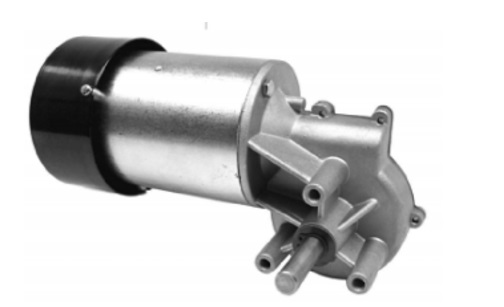
\includegraphics{figuras/Motor.jpg}
  \caption{Foto ilustrativa do motor utilizado no projeto.}
\end{figure}

\subsection{Dimensionamento do Motor}

O dimensionamento do motor foi realizado de acordo com o equacionamento e os dados obtidos do fornecedor a seguir.

O modelo do motor utilizado é o MR 210 VER 240, com tensão de 12V, fabricado
pela Motron, e como a redução utilizada (sistema de transmissão) é de 6 para 1,
a partir dos dados do motor é possível calcular a carga nominal do conjunto
cadeira e usuário.

\[\frac{n_1}{n_2} = \frac{d_1}{d_2} = \frac{T_1}{T_2}\]

\[T_2 = 6* T_1 \]

Torque nominal de um motor = 24 Nm

Aplicando a relação de transmissão, o torque na roda movida é:

\[T_2 = 6* T_1  = 6*24 = 144 Nm\]

A força aplicada na roda movida, com raio de 0,3m, é dado por:

\[\frac{n_1}{n_2} = \frac{T_2}{R} = \frac{144}{0.3} = 480 N\]

Então a força aplicada nas duas rodas é igual a 960 N.

A força necessária para mover a cadeira em uma superfície horizontal plano é dada pela seguinte equação:

\[F = F_a + F_r\]

Onde \(F_a\) é a força de aceleração e \(F_r\)  é a força de resistência causada pelo atrito estático.

\[F_a = M*a\]
\[F_R = M*g*\mu\]

A Rotação nominal do motor é de 215 RPM, usando a relação de transmissão a rotação da roda movida é reduzida seis vezes, então \(n_2\) = 35,84 RPM. A partir do valor de \(n_2\) e do raio da roda é possível encontrar sua velocidade linear.

\[V_2 = 35.84 * \frac{2*\pi}{60}*0.3\ = 1.1 m/s\] 

A partir do tempo de 4 segundos definido para se alcançar a velocidade máxima é possível calcular a aceleração da cadeira.

\[a = \frac{1.1}{4} = 0.28 m/s^2\]

A partir da equação para força movida é possível encontrar a massa que os motores poderão mover.

\[960 = M*a + M*g*\mu = 0.28M + 2.94M\]
\[M = \frac{960}{3.22} = 298 Kg\]

\section{Dimensionamento da bateria}

O dimensionamento da bateria foi realizado de acordo com o equacionamento e
os dados obtidos a partir das figuras a seguir.

\begin{figure}[h!]
  \centering
  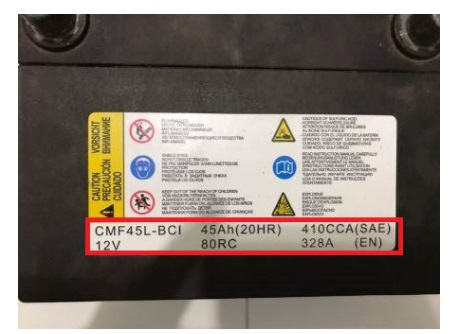
\includegraphics{figuras/Bateria1.jpg}
  \caption{Dados da bateria usada no projeto.}
\end{figure}

\begin{figure}[h!]
  \centering
  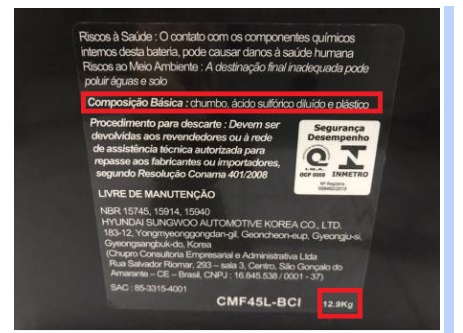
\includegraphics{figuras/Bateria2.jpg}
  \caption{Dados da bateria usada no projeto.}
\end{figure}

Foi definido que para fins de teste e apresentação o tempo de funcionamento da cadeira será de 15 minutos, com essa informação e a corrente nominal do sistema, de 24 A, é possível estimar a bateria necessária. 

\[M = 24*0.25 = 6 Ah\]

O grupo adquiriu uma bateria automotiva de 45 Ah para ser utilizada nos testes, o que é mais de sete vezes maior do que a bateria dimensionada.

\section{Carregador para bateria}

 Um carregador constitui-se de uma fonte que estabelece uma corrente em sentido contrário na célula, pilha ou bateria que se deseja carregar. O conceito em volta de se recarregar uma bateria é bastante simples: ao passar pela substância fornecedora de energia uma corrente no sentido contrário àquela que ela fornece normalmente, a reação se inverte e a substância "absorve" a energia liberada, voltando à sua condição inicial. (BAHIA, 2015)

A recarga da bateria pode ser feita de forma rápida ou lenta. A carga rápida ou lenta nada mais é do que o nível de corrente aplicado numa bateria para atingir o seu nível de carga num determinado tempo. A carga rápida consiste em aplicar níveis de correntes elevados para reduzir o tempo de recarga. A elevação da corrente provoca superaquecimento da bateria e em consequência reduz significativamente a sua vida útil. Este tipo de recarga rápida não é recomendado. O sistema recomendado para a recarga de baterias é o de carga lenta, pois o de carga rápida provoca muitos danos à bateria e por isso, não deve ser utilizado. Para isso, recomenda-se utilizar como corrente de recarga mínima de 5\% e máxima de 10\% da capacidade nominal em Ah da bateria. (SOARES et al., 2012)

Tendo em vista a bateria escolhida para o projeto, que possui 45Ah de capacidade nominal, o carregador desenvolvido para a mesma deve fornecer corrente de recarga de aproximadamente 4,5A por volta de 10h. Como já explicitado, esse tempo se faz necessário para que a vida útil da bateria não seja comprometida. Dessa forma, de acordo com a disponibilidade de componentes encontrados no mercado, para a confecção do carregador, foi possível desenvolvê-lo de tal forma a fornecer 5A de corrente de recarga, diminuindo então, o tempo de recarga para 9h. Assim sendo, o carregador proposto foi desenvolvido seguindo as orientações descritas nos circuitos ilustrados nas \textbf{\textit{FIGURAS 6 e 7}}, utilizando os seguintes materiais:

\begin{itemize}
\item 1 transformador (entrada 110/220V, saída 15V 5ª); 
\item 1 ponte retificadora 10A;
\item fios vermelho e preto;
\item 2 garras modelo “jacaré” (1 vermelho e 1 preto);
\item 1 cabo de força;
\item 1 fusível 10A;
\item 1 porta fusível; 
\item 1 LED; 
\item 1 resistor de 1K\(\Omega\) ; 
\item botão de liga desliga e caixa de madeira.
\end{itemize}

\newpage

\begin{figure}[h!]
  \centering
  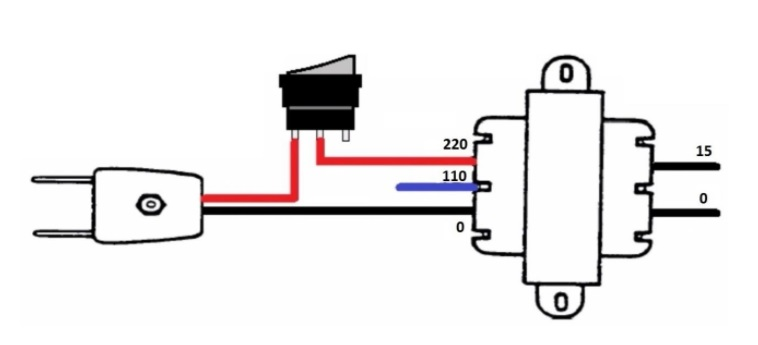
\includegraphics{figuras/Transformador1.jpg}
  \caption{Circuito de entrada do transformador.}
\end{figure}

\begin{figure}[h!]
  \centering
  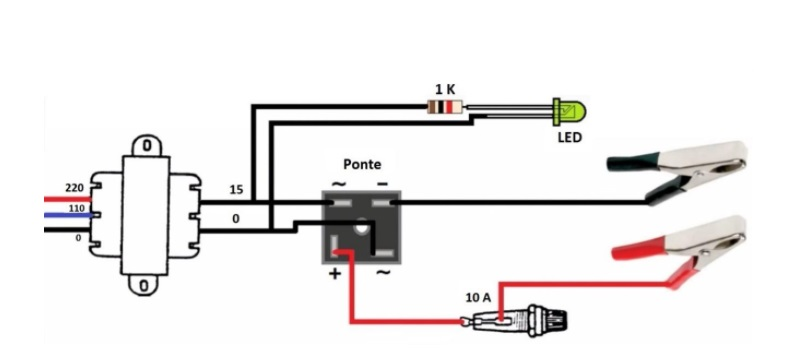
\includegraphics{figuras/Transformador2.jpg}
  \caption{Circuito de saída do transformador.}
\end{figure}

Durante o carregamento da bateria, com o auxílio de um multímetro, pode-se
observar que a tensão em seus terminais irá aumentar gradativamente, quando
esse aumento gradativo cessar significará que a bateria estará totalmente
carregada. Para determinar esse valor em que a tensão irá parar de aumentar,
deve-se aplicar a seguinte razão: 

\[V_{CC} = V_{CA}*\sqrt[]{2} - V_D\]

Onde: 


\begin{itemize}
\item \(V_{CC}\) – Tensão máxima na bateria
\item \(V_{CA}\)– Tensão alternada que sai do transformador
\item \(V_{D}\) – Perda existente na ponte retificadora
\end{itemize}

O transformador utilizado tem saída de aproximadamente 15 V RMS, equivalente a
21 V de pico, dessa forma a tensão se torna excessiva para a carga da bateria:

\[V_{CC} = 14.8 * \sqrt[]{2} - 1.4\]

\[V_{CC} = 19.6 V\]

Para solucionar esse problema, um regulador de tensão será acoplado após a
ponte retificadora, garantindo que a saída do carregador seja sempre cerca
de 15 V. Portanto, após aproximadamente 9h, e constatado por volta de 15 V
nos terminais da bateria em processo de carregamento, a bateria pode ser
considerada totalmente carregada.

\section{Controle PWM e Ponte H}

Para o controle do motor através de um \textit{joystick} foi projetado e
implementado um \textit{driver} que consiste basicamente de quatro partes para
seu funcionamento, sendo elas: Circuito de chaveamento, ponte H, dobrador de
tensão e o código de controle.

\subsection{Circuito de Chaveamento}

\begin{figure}[h!]
  \centering
  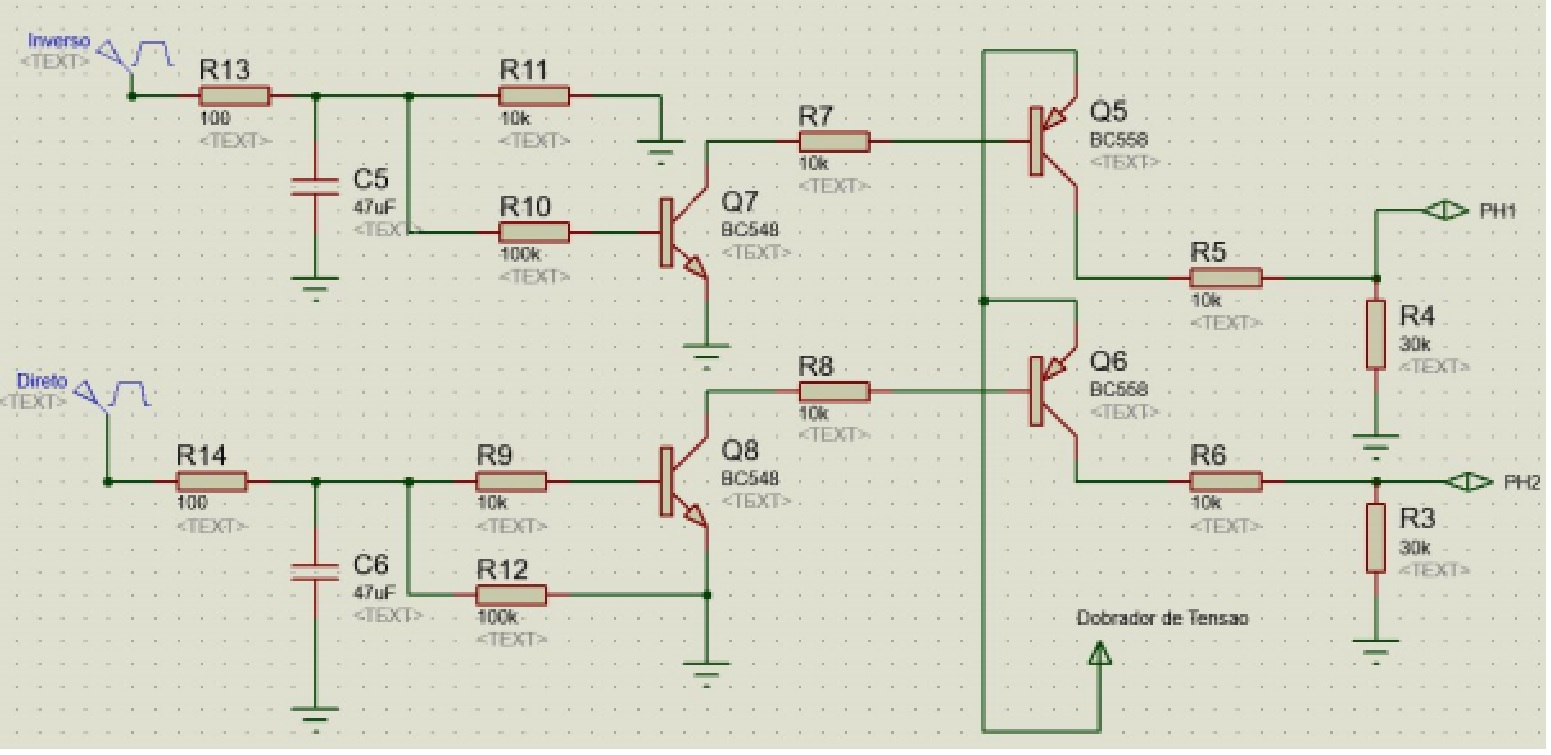
\includegraphics[width=1.0\textwidth]{figuras/Chaveamento.jpg}
  \caption{Circuito de Chaveamento.}
\end{figure}

A figura acima ilustra o circuito de chaveamento, o qual é responsável por chavear as entradas do PWM com a ponte H e indicar ao circuito para qual sentido o motor deve rodar, seja ela no seu sentido direto ou inverso. O circuito projetado funciona da seguinte maneira:

\begin{itemize}
	\item Para que ocorra passagem de corrente nos transistores Q5 e Q6 é
        necessário que os transistores Q7 e Q8 estejam em saturação e,
        portanto, quando em corte, nenhum dos transistores é capaz de
        transmitir corrente;
	\item Os capacitores C6 e C5 e os resistores R13 e R14 funcionam como
        filtros passa-baixa que são responsáveis por obter a tensão analógica
        para o PWM;
    \item Com a tensão dos PWMs obtida ocorrerá a saturação de Q7 e Q8 ou não,
        depende dos valores que forem entrados pelo PWM. Suponha-se que a
        tensão do PWM Direto entre com 5V e o PWM Inverso com 0V, apenas o
        transistor Q8 estará em saturação, deixando que exista corrente apenas
        entre o coletor e emissor de Q8, sendo Q7 em corte e sem corrente. 
    \item Os transistores Q5 e Q6 recebem em seu emissor uma tensão dobrada da
        fonte de tensão, a necessidade de uma tensão dobrada vai ser explicada
        mais adiante. Quando Q7 e Q8 estão em saturação ocorre então uma
        saturação também nos transistores Q5 e Q6, existindo então uma passagem
        de corrente entre o emissor-coletor de Q5 e Q6. Pegando a mesma
        suposição feita no item acima, Q5 permanece em corte e portanto sem
        corrente para a saída PH2, gerando assim uma tensão de 0V, no passo que
        Q6 em saturação permite a passagem de corrente entre emissor-coletor e
        PH1 tem sua saída determinada pelo divisor de tensão R6 e R3.
    \item As saídas PH1 e PH2 são as saídas que são ligadas a ponte H para que
        o motor possa girar no sentido desejado.
\end{itemize}

O teste do circuito de chaveamento foi feito em conjunto do circuito de
dobrador de tensão, explicado mais à frente, os circuitos foram montados em uma
placa \textit{protoboard}. Posteriormente, para se instalar na cadeira, os
circuitos serão feitos em placas de circuito impresso (PCB). A imagem abaixo
ilustra o circuito de teste montado.

\begin{figure}[h!]
  \centering
  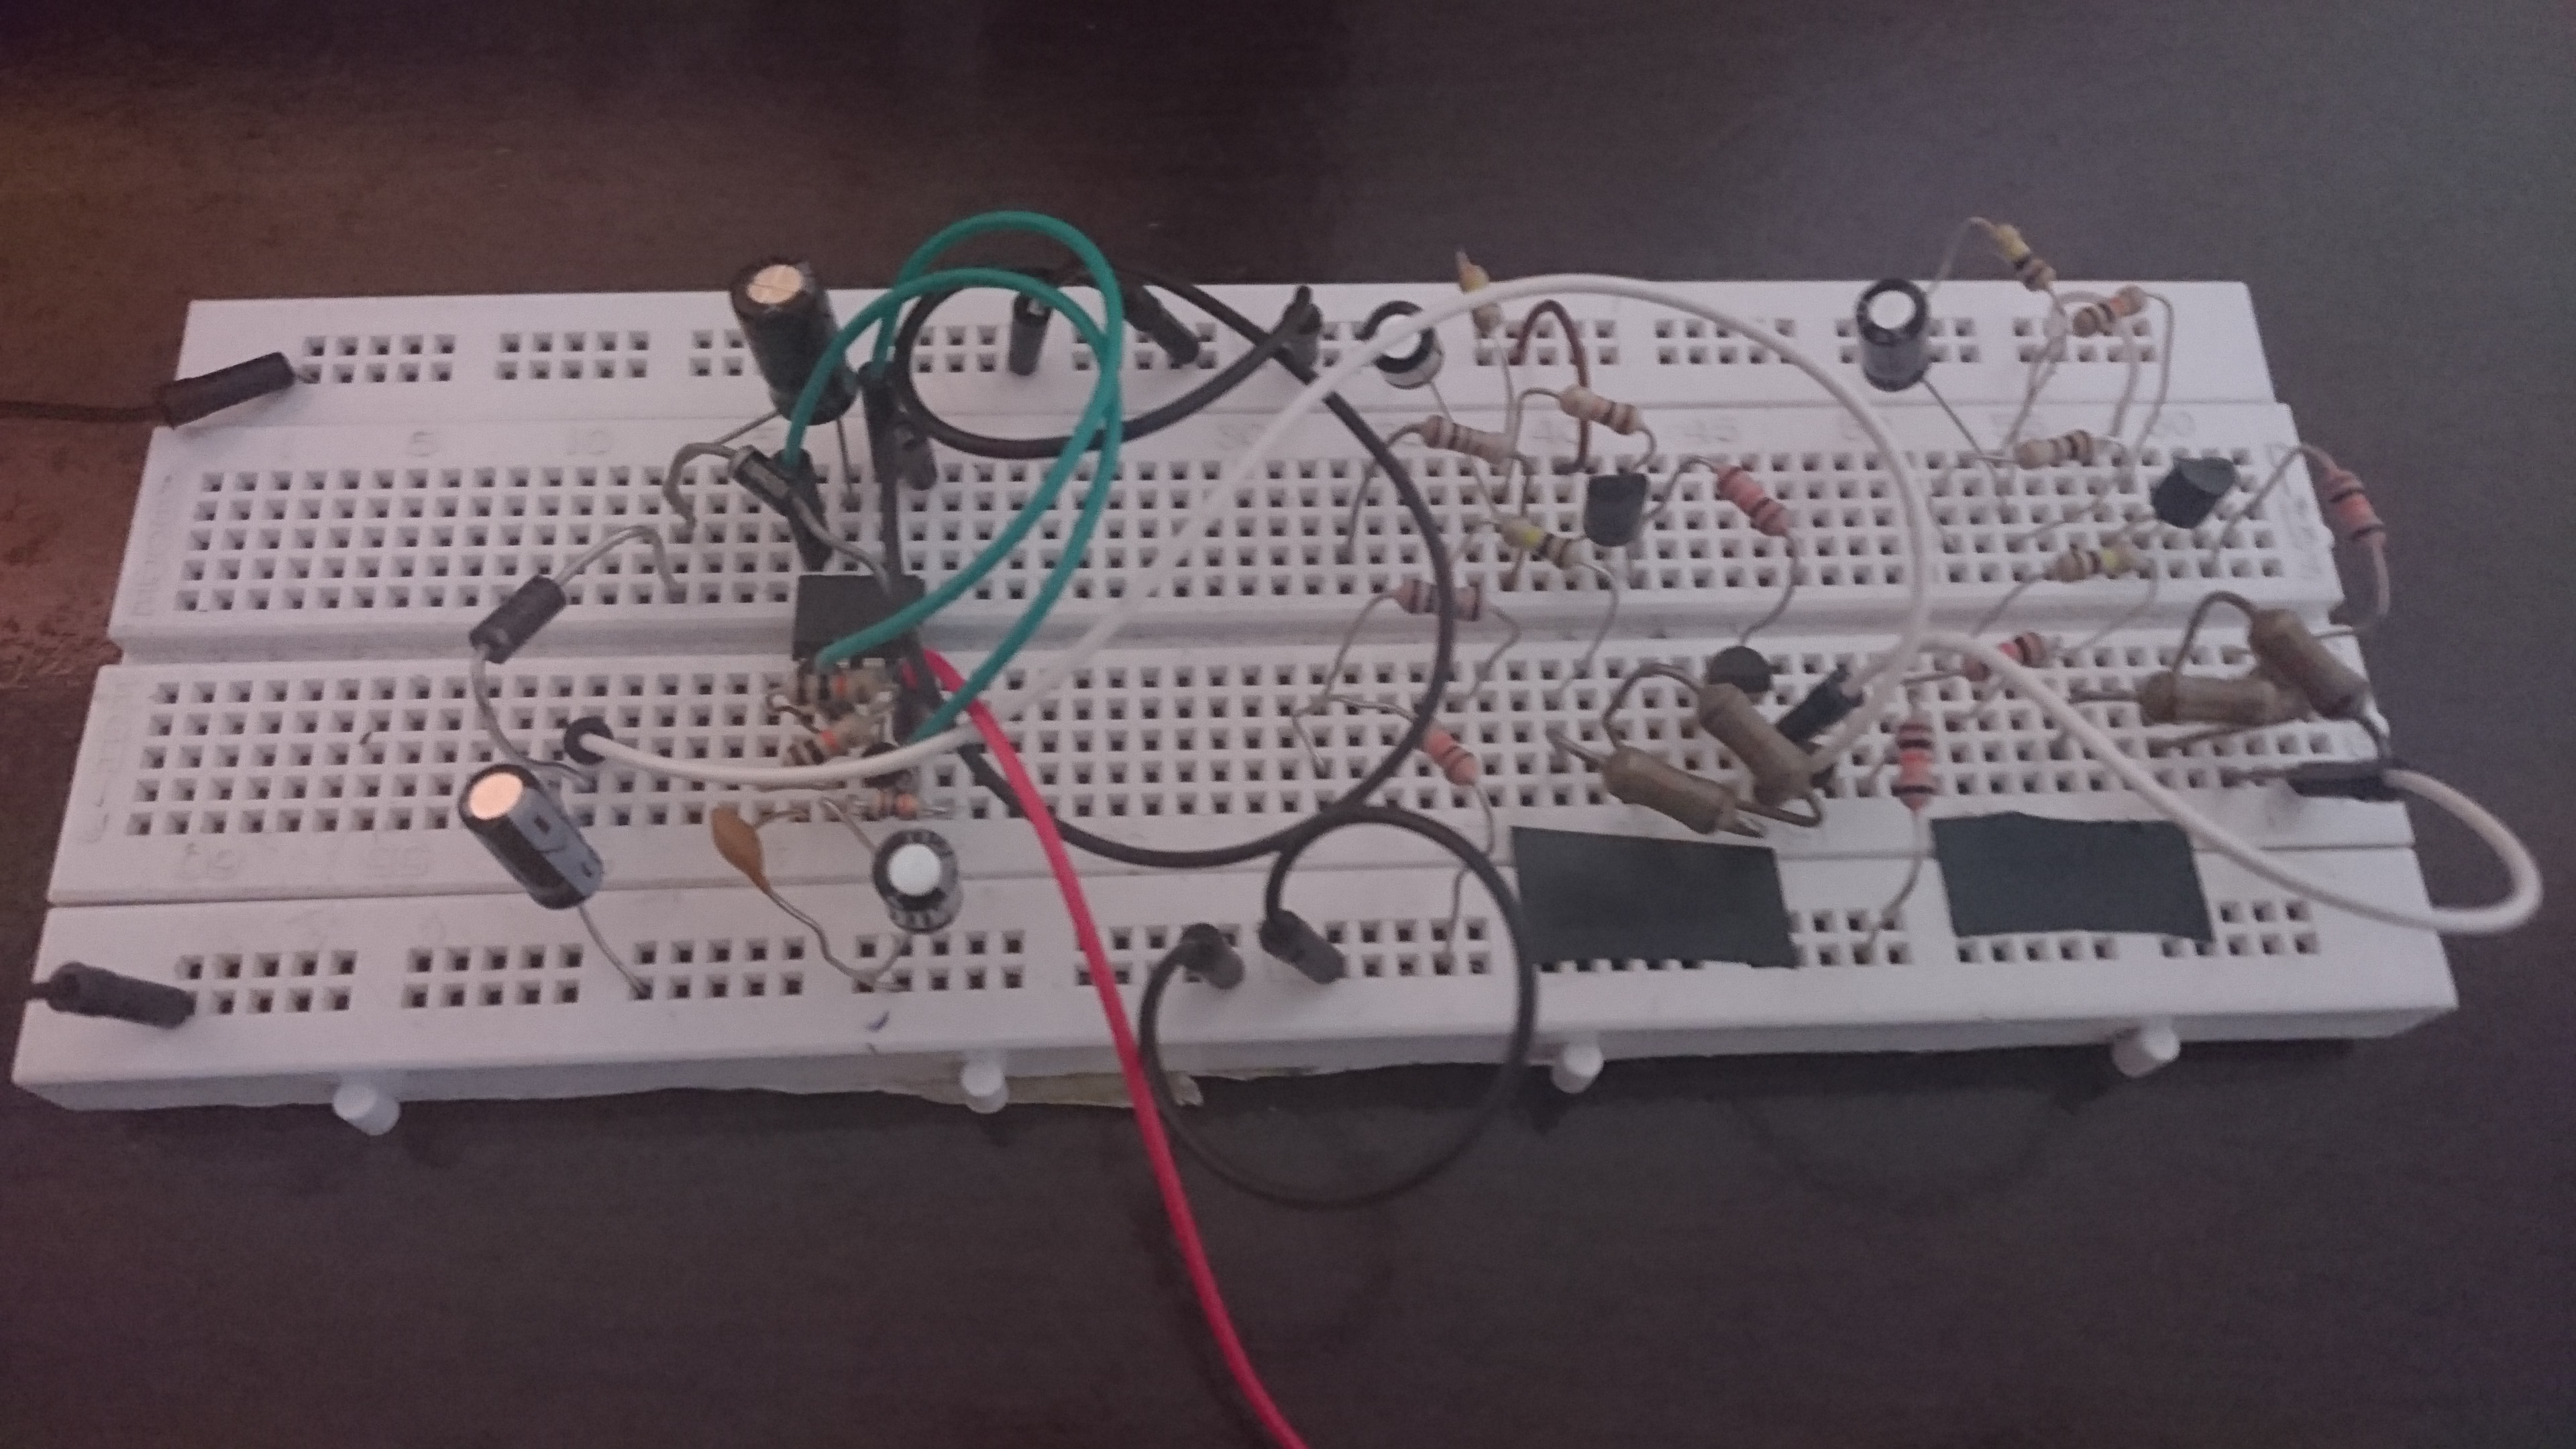
\includegraphics[width=1.0\textwidth]{figuras/TesteChaveamento.JPG}
  \caption{Circuito de chaveamento (à direita) e circuito dobrador de tensão (à esquerda).}
\end{figure}
\newpage
\subsection{Ponte H}

A ponte H é responsável por fazer os motores girarem para os sentidos desejados, ou seja, sentido direto ou sentido inverso. A figura abaixo ilustra a ponte H realizada.

\begin{figure}[h!]
  \centering
  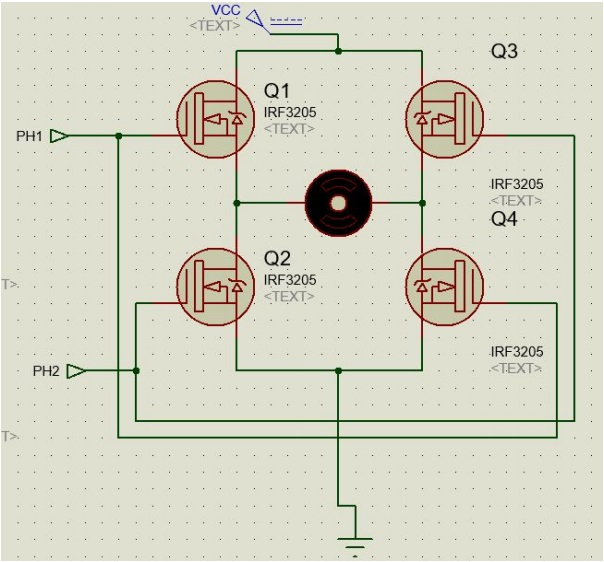
\includegraphics{figuras/Ponte_H.jpg}
  \caption{Ponte H.}
\end{figure}

A ponte H projetada funciona da seguinte maneira: 

\begin{itemize}
	\item Os transistores Q1 e Q3 recebem no seu terminal DRAIN a tensão da bateria de 12V e no seu terminal GATE a tensão advinda do chaveamento da parte 1. Para que exista corrente entre os terminais DRAIN e SOURCE os transistores devem estar em saturação e, portanto, a tensão que chega ao GATE desses transistores para que possa estar em saturação e entregar ao motor 12V exigidos pelo mesmo em seu terminal SOURCE, deve ser uma tensão de 12V + 4.5V, pois 12V é a tensão entregue pelo terminal SOURCE e 4.5V é a tensão de limiar do transistor IRF3205 em uso, ou seja, para o correto funcionamento dos transistores Q1 e Q3 é necessário que uma tensão de 16.5V seja entregue por PH1 e PH2.
    \item O dobrador de tensão serve para dar essa tensão a mais que a tensão entregue pela bateria, pois 12 V não seriam o suficiente para que os motores girassem em sua plenitude visto que o terminal GATE de Q1 e Q3 necessitam de 16.5 V.
    \item Os transistores Q2 e Q4 sao os transistores responsáveis por ligar a ponte H ao terra do circuito, possibilitando a passagem de corrente pelos motores. 
    \item Os transistores Q1 e Q4 sao curto-circuitados e Q2 e Q3 também. Estas ligações são as responsáveis por dizer o sentido da corrente e portanto o sentido que o motor vai girar. Quando Q1 e Q4 recebem 16.5V em seu GATE e Q2 e Q3 0V em seu GATE, aqueles entram em saturação enquantos estes entram em corte fazendo com que a corrente percorra o sentido esquerda-direita. Já quando o contrário ocorre e Q2 e Q3 estão em saturação e Q1 e Q4 em corte, a corrente percorre o sentido direita-esquerda. 
    \item A condição dos 4 transistores estarem em saturação deve ser evitada ou melhor, não deve ocorrer, uma vez que os transistores podem superaquecer enfrentando problemas para o circuito, portanto esta condição foi pensada e efetuada nos controles de PWM.

\end{itemize}

A placa de testes da ponte H pode ser vista na imagem abaixo. A montagem da
mesma foi feita em uma placa de fenolite furada, de 10x10 cm, com os
componentes soldados e com as conexões realizadas utilizando fios de cobre com
6.5 \(mm^2\) de seção nominal, que são suficientes para correntes de até 80 A
de acordo com as legislações atuais. A placa final à ser instalada na cadeira
será feita com placas de circuito impresso, atentando ao fato de que suas
trilhas devem suportar correntes de até 50 A.

\begin{figure}[h!]
  \centering
  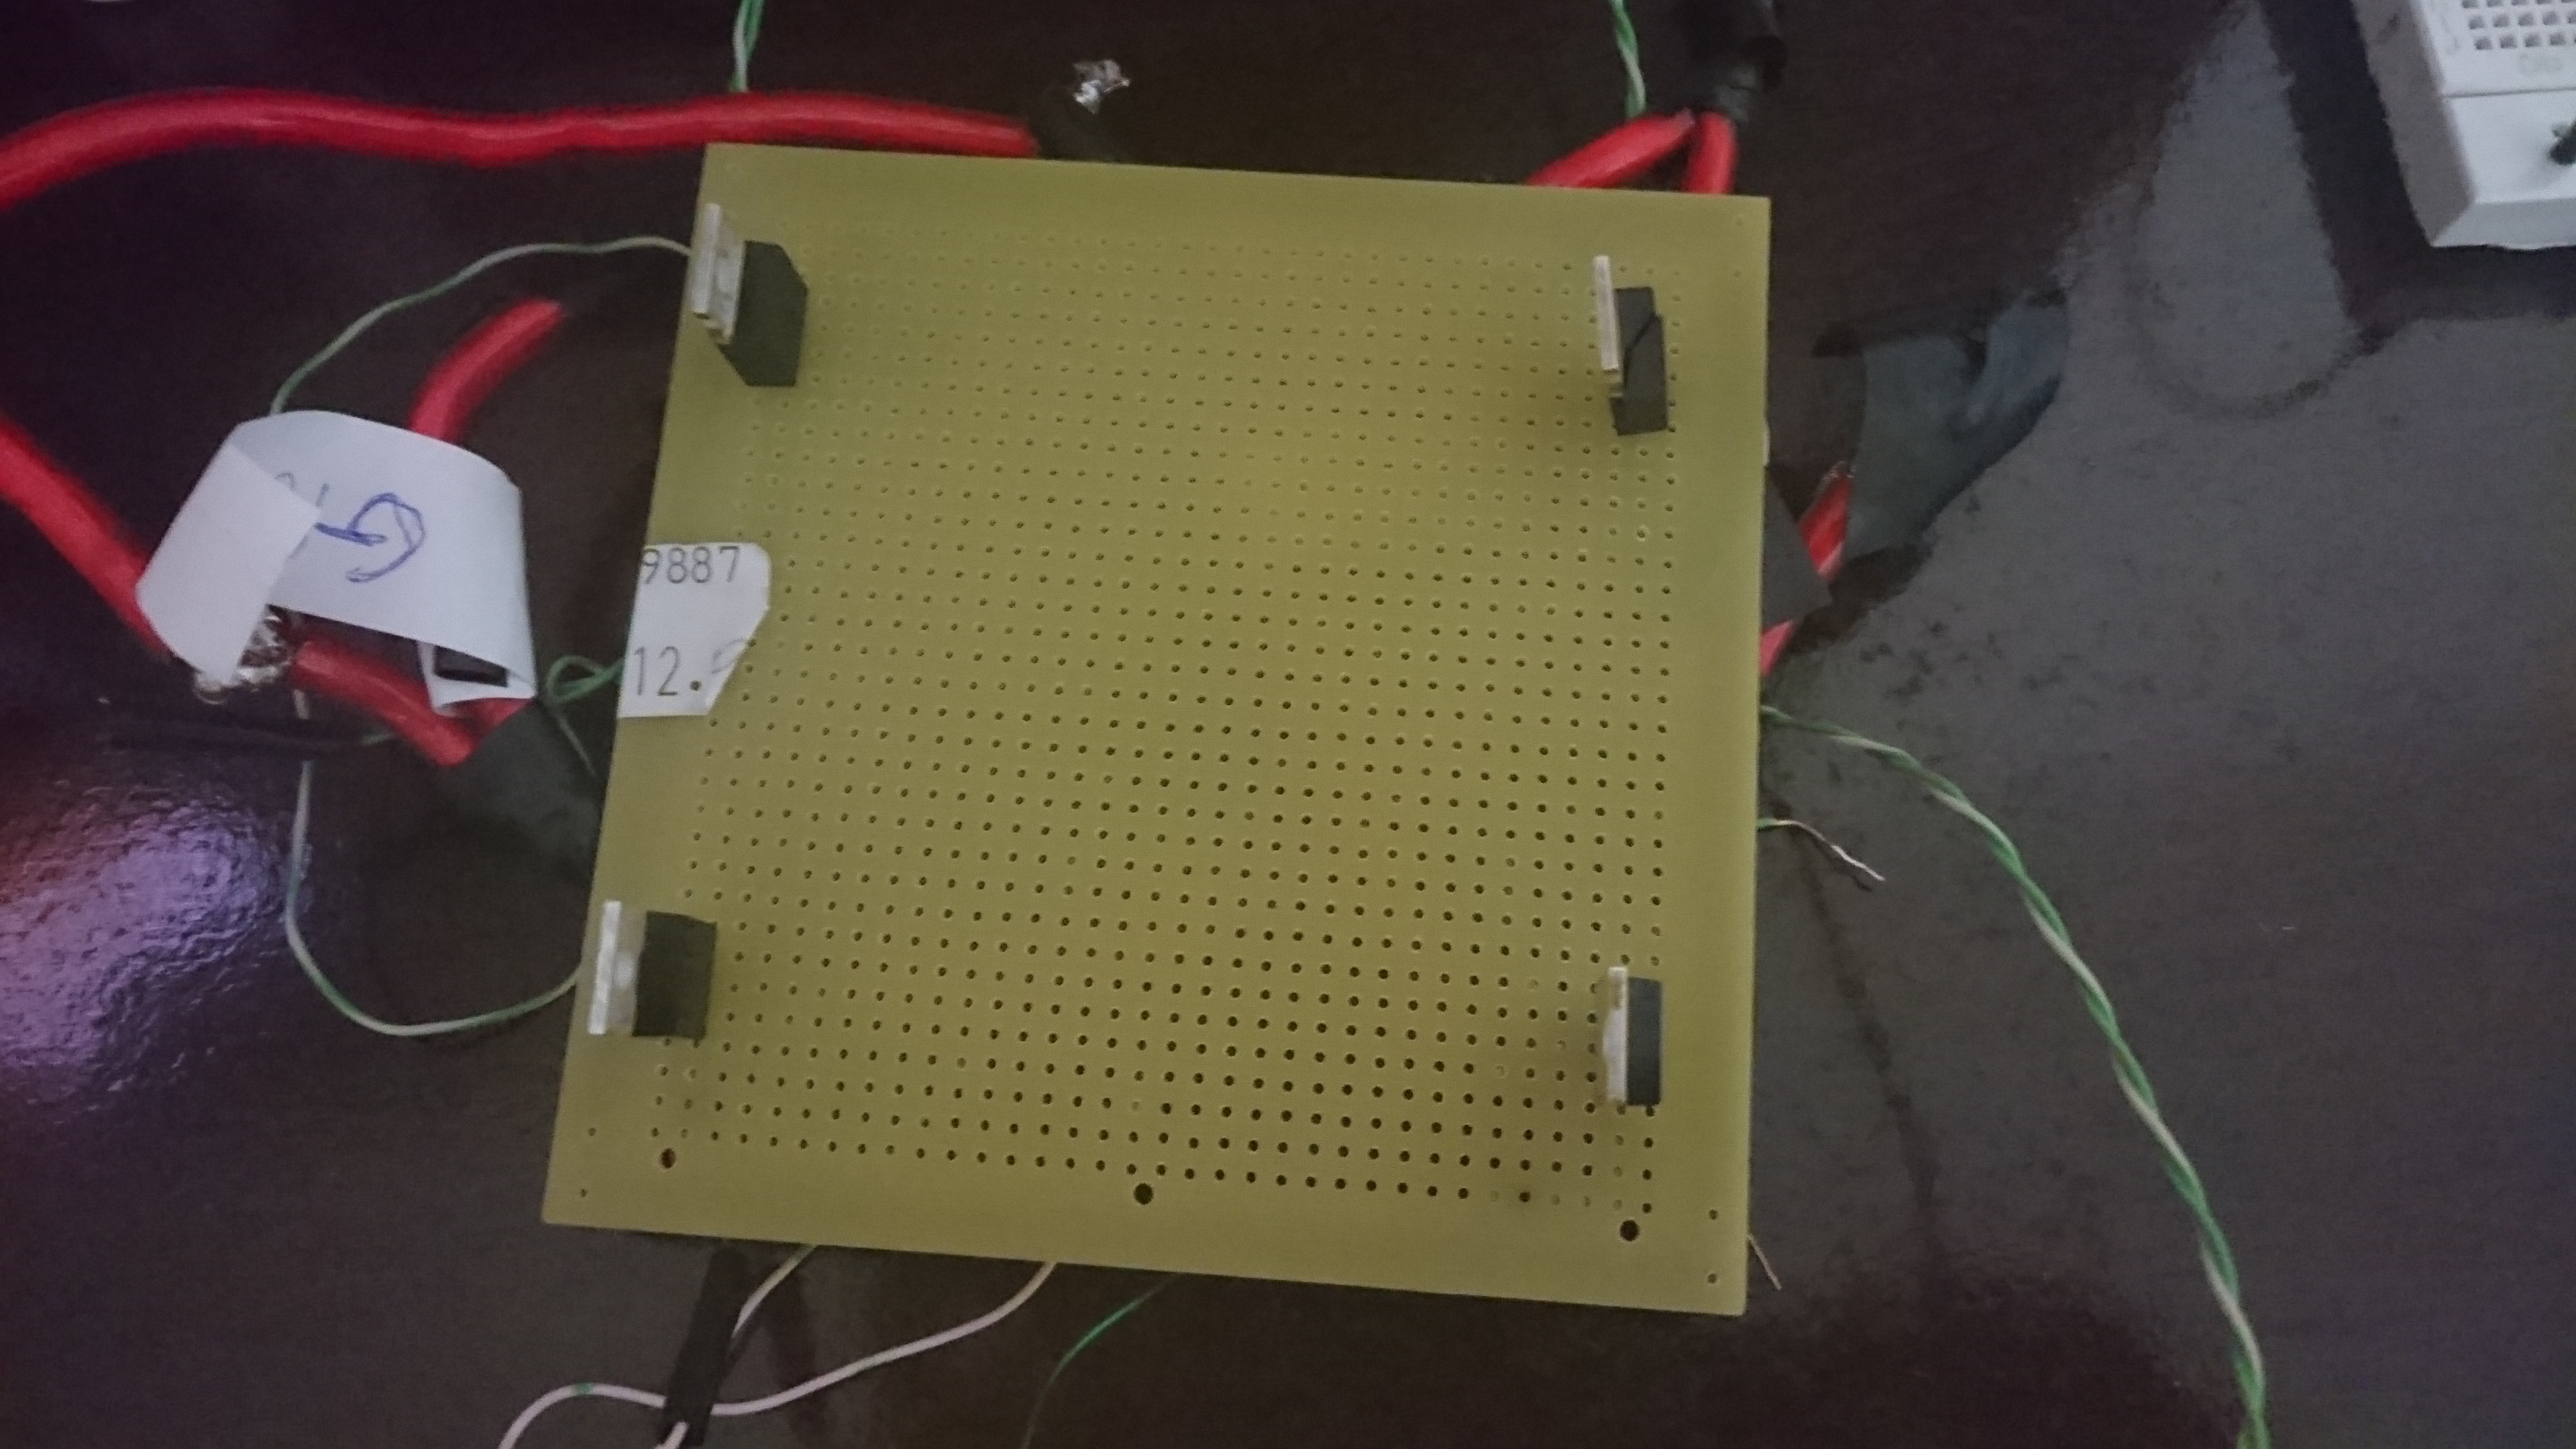
\includegraphics[width=1.0\textwidth]{figuras/TestePonteH.JPG}
  \caption{Placa de teste da ponte H.}
\end{figure}

\subsection{Dobrador de tensão}

O circuito dobrador de tensão, como dito anteriormente, é necessário para
realizar o chaveamento do circuito. O dobrador foi realizado utilizando o CI
555 em sua configuração astável. A figura abaixo ilustra o circuito do dobrador de tensão

\begin{figure}[h!]
  \centering
  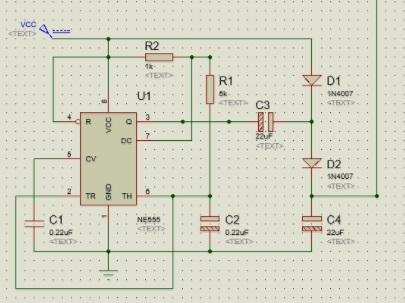
\includegraphics[width=1.0\textwidth]{figuras/Dobrador.jpg}
  \caption{Circuito do dobrador de tensão.}
\end{figure}

\subsection{Controlador PWM - Software}

Para se controlar os motores através do \textit{joystick}, foi utilizado um
microcontrolador Arduino Nano. 

O \textit{joystick} é constituído de 2 potenciômetros que têm seus valores
analógicos medidos pelo Arduíno. Em seu ponto inicial, os valores digitais do eixo x e y
do \textit{joystick} são, respectivamente, 511 e 491. Na direção positiva, os valores de
y e x diminuem até chegarem à 0 em seu limite positivo, já na direção negativa,
os valores aumentam até chegarem à 1024, em seu limite negativo. A figura
abaixo mostra o \textit{joystick} e o Arduíno utilizados

O sinal de PWM é gerado utilizando os timers do Arduíno. Cada motor possui 2 pulsos PWM (um para controlar a corrente no sentido direto e outro para o inverso), assim sendo, são necessários 4 timers para o controle total da cadeira. No código, os timers utilizados foram os TCCR1A, TCCR1B, TCCR2A, TCCR2B. O dutycicle dos PWMs pode ser modificados de acordo com o valor inserido em sua função, com 255 sendo 100\% de DutyCycle e 0 sendo 0\%.

\begin{figure}[h!]
  \centering
  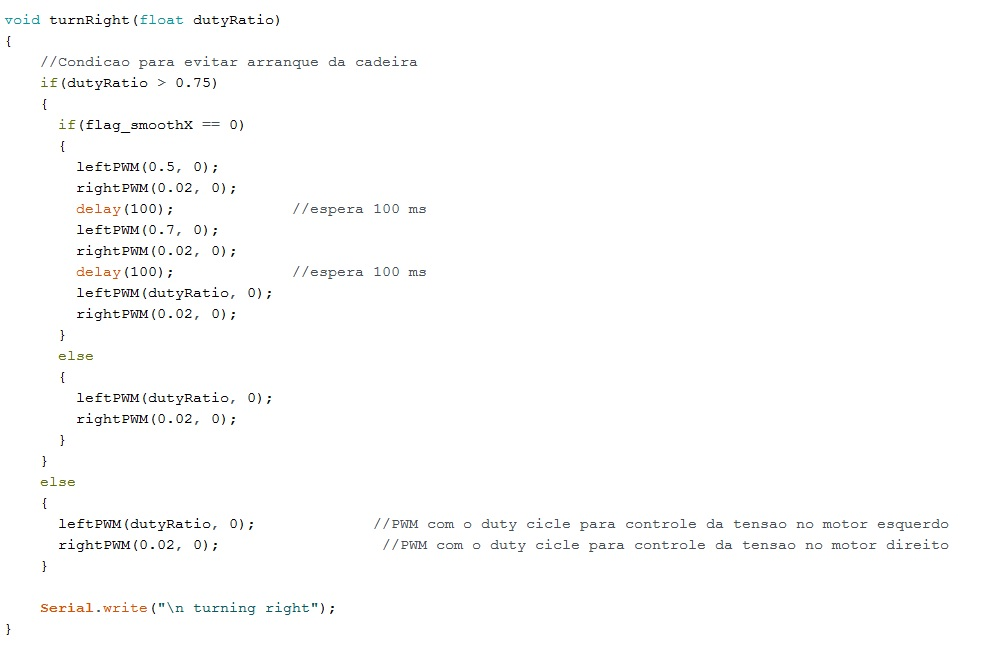
\includegraphics[width=1.0\textwidth]{figuras/Funcoes.jpg}
  \caption{Exemplo de função usado no controle PWM.}
\end{figure}

Foram criadas funções para os movimentos da cadeira (parado, frente, trás, curva à direita e curva à esquerda). Essas funções são chamadas quando executadas pelo usuário no joystick, através de lógica condicional. Também é modificado o DutyCycle do PWM de acordo com a intensidade do comando no joystick. Um exemplo de função pode ser visto na figura acima.

Há também condições para garantir que a cadeira não dê uma aceleração súbita, evitando assim riscos de quedas por parte do usuário. Essas funções garantem que, ao acionar os motores com força acima de 75\% saindo do repouso, os sinais de PWM aumentem seus dutycyles pausadamente, indo de 0\% a 50\%, de 50\% a 70\% e de 70\% até o valor selecionado originalmente, com intervalos entre os acréscimos.

